\documentclass[twoside]{book}

% Packages required by doxygen
\usepackage{calc}
\usepackage{doxygen}
\usepackage{graphicx}
\usepackage[utf8]{inputenc}
\usepackage{makeidx}
\usepackage{multicol}
\usepackage{multirow}
\usepackage{textcomp}
\usepackage[table]{xcolor}

% NLS support packages
\usepackage[french]{babel}

% Font selection
\usepackage[T1]{fontenc}
\usepackage{mathptmx}
\usepackage[scaled=.90]{helvet}
\usepackage{courier}
\usepackage{amssymb}
\usepackage{sectsty}
\renewcommand{\familydefault}{\sfdefault}
\allsectionsfont{%
  \fontseries{bc}\selectfont%
  \color{darkgray}%
}
\renewcommand{\DoxyLabelFont}{%
  \fontseries{bc}\selectfont%
  \color{darkgray}%
}

% Page & text layout
\usepackage{geometry}
\geometry{%
  a4paper,%
  top=2.5cm,%
  bottom=2.5cm,%
  left=2.5cm,%
  right=2.5cm%
}
\tolerance=750
\hfuzz=15pt
\hbadness=750
\setlength{\emergencystretch}{15pt}
\setlength{\parindent}{0cm}
\setlength{\parskip}{0.2cm}
\makeatletter
\renewcommand{\paragraph}{%
  \@startsection{paragraph}{4}{0ex}{-1.0ex}{1.0ex}{%
    \normalfont\normalsize\bfseries\SS@parafont%
  }%
}
\renewcommand{\subparagraph}{%
  \@startsection{subparagraph}{5}{0ex}{-1.0ex}{1.0ex}{%
    \normalfont\normalsize\bfseries\SS@subparafont%
  }%
}
\makeatother

% Headers & footers
\usepackage{fancyhdr}
\pagestyle{fancyplain}
\fancyhead[LE]{\fancyplain{}{\bfseries\thepage}}
\fancyhead[CE]{\fancyplain{}{}}
\fancyhead[RE]{\fancyplain{}{\bfseries\leftmark}}
\fancyhead[LO]{\fancyplain{}{\bfseries\rightmark}}
\fancyhead[CO]{\fancyplain{}{}}
\fancyhead[RO]{\fancyplain{}{\bfseries\thepage}}
\fancyfoot[LE]{\fancyplain{}{}}
\fancyfoot[CE]{\fancyplain{}{}}
\fancyfoot[RE]{\fancyplain{}{\bfseries\scriptsize Généré le Jeudi 15 Mai 2014 14\-:52\-:18 pour I\-G\-Osat Simulator par Doxygen }}
\fancyfoot[LO]{\fancyplain{}{\bfseries\scriptsize Généré le Jeudi 15 Mai 2014 14\-:52\-:18 pour I\-G\-Osat Simulator par Doxygen }}
\fancyfoot[CO]{\fancyplain{}{}}
\fancyfoot[RO]{\fancyplain{}{}}
\renewcommand{\footrulewidth}{0.4pt}
\renewcommand{\chaptermark}[1]{%
  \markboth{#1}{}%
}
\renewcommand{\sectionmark}[1]{%
  \markright{\thesection\ #1}%
}

% Indices & bibliography
\usepackage{natbib}
\usepackage[titles]{tocloft}
\setcounter{tocdepth}{3}
\setcounter{secnumdepth}{5}
\makeindex

% Hyperlinks (required, but should be loaded last)
\usepackage{ifpdf}
\ifpdf
  \usepackage[pdftex,pagebackref=true]{hyperref}
\else
  \usepackage[ps2pdf,pagebackref=true]{hyperref}
\fi
\hypersetup{%
  colorlinks=true,%
  linkcolor=blue,%
  citecolor=blue,%
  unicode%
}

% Custom commands
\newcommand{\clearemptydoublepage}{%
  \newpage{\pagestyle{empty}\cleardoublepage}%
}


%===== C O N T E N T S =====

\begin{document}

% Titlepage & ToC
\hypersetup{pageanchor=false}
\pagenumbering{roman}
\begin{titlepage}
\vspace*{7cm}
\begin{center}%
{\Large I\-G\-Osat Simulator }\\
\vspace*{1cm}
{\large Généré par Doxygen 1.8.6}\\
\vspace*{0.5cm}
{\small Jeudi 15 Mai 2014 14:52:18}\\
\end{center}
\end{titlepage}
\clearemptydoublepage
\tableofcontents
\clearemptydoublepage
\pagenumbering{arabic}
\hypersetup{pageanchor=true}

%--- Begin generated contents ---
\chapter{Référence Génerateur des classes}
\label{docGenereateur}
\hypertarget{docGenereateur}{}
\hypertarget{docGenereateur_objectif}{}\section{Les objectifs}\label{docGenereateur_objectif}
Pour faciliter la création des nouveaux modules, le script de générateur des modules est proposé. Il permet de créer une classe de base d'un Module/\-Macro\-Module et un fichier X\-M\-L avec la configuration de ce \hyperlink{classModule}{Module}. Ce script est écrit en langage Python, il faut donc avoir l'interprète de Python installé sur votre ordinateur.\hypertarget{docGenereateur_manuel}{}\section{Manuel de création d'un module}\label{docGenereateur_manuel}
Le script de génération des modules se trouve dans le répertoire Projet\-\_\-\-Simulateur\-\_\-\-I\-G\-O\-S\-A\-T/\-I\-G\-Ogen/src/. Pour le lancer, saisissez \char`\"{}python I\-G\-Ogen.\-py\char`\"{} dans la console en se trouvant dans un bon repertoire. Vous allez voir des options intuitives\-:

$>$Choisissez une composante à créer\-: $>$\mbox{[}1\mbox{]} \-: \hyperlink{classModule}{Module} $>$\mbox{[}2\mbox{]} \-: Macromodule

Alors, vous choisissez ce que vous voulez créer. Au niveau de génération, la seule difference entre \hyperlink{classModule}{Module} et \hyperlink{classMacroModule}{Macro\-Module}, c'est une classe qui sera generée. Puis, le script vous demande de tapez le nom d'un module. Soyez attentif au choix de ce nom, vu que ce sera le nom de classe. En accord avec la convention, on donne un nom simple au Macromodule (par exemple \hyperlink{classBattery}{Battery}, Antenne, G\-P\-S) et un nom composé avec $\ast$\-Module à la fin (par exemple Antenne\-Recepteur\-Module) pour les modules atomiques. (vous pouvez toujours changer cette convention si celui-\/ci ne vous convient pas).

Puis, le script vous demande de tapez le chemin vers un fichier .X\-M\-L. Si vous voulez que votre fichier module1.\-xml se trouve dans un repertoire config/\-Module1 de simulateur, tapez \char`\"{}\-Module1/module1.\-xml\char`\"{}.

Puis, il vous sera proposé d'ajouter des composantes. Vous pouvez ajouter au module un message, un socket ou un paramètre. Suivez les instructions. Après chaque ajoute d'un composante vous serez retourné au menu principal d'ajoute des composantes.

Une fois que vous avez fini, choississez les options 4 et 5 pour générer un fichier .X\-M\-L et des fichiers de classe .cpp et .h. Après avoir fait tout ça, quittez le script.\hypertarget{docGenereateur_resultat}{}\section{Le resultat de génération}\label{docGenereateur_resultat}
Après avoir un script executé, vous allez trouver dans le repertoire \char`\"{}\-Projet\-\_\-\-Simulateur\-\_\-\-I\-G\-O\-S\-A\-T/\-I\-G\-Ogen/src/\char`\"{} les fichiers .cpp et .h de classe d'un nouveau module et soit un nouveau repertoire que vouz avez indiqué comme le repertoire contenant fichier .X\-M\-L, soit un fichier .X\-M\-L tout seul si vous n'avez indiqué qu'un nom de fichier.\hypertarget{docGenereateur_apres}{}\section{Qu'est-\/ce que je fais après?}\label{docGenereateur_apres}
Mettez le fichier de classe dans un bon repertoire de votre projet. Soyez vigilant avec la structure de votre projet pour ne pas la rendre décharge. Puis, il vous faut bien placer un fichier .X\-M\-L. Si le repertoire que vous avez choisi existe déjà dans le repertoire \char`\"{}config/\char`\"{}, juste remplacer un fichier .X\-M\-L dans un bon repertoire là-\/bas. Sinon, remplacez le repertoire entier à \char`\"{}config/\char`\"{}. Pour tester le résultat, créez votre nouveau \hyperlink{classModule}{Module} quelque part dans le projet et essayez de le compiler. Si le projet compile bien et vous n'avez pas des warnings dans la console à cause de fichier .X\-M\-L introuvable, alors vous avez tout bien fait. Maintenant, il est le temps de remplir ce nouveau module par fonctionnalité non-\/générique. 
\chapter{Référence Création Macro-\/\-Module}
\label{docMacroModule}
\hypertarget{docMacroModule}{}
\hypertarget{docModule_classCreation}{}\section{Creation d'un nouveau classe}\label{docModule_classCreation}
Pour créer un nouveau macro-\/module, il faut hériter une nouvelle classe de classe \hyperlink{classMacroModule}{Macro\-Module} qui va représenter votre nouveau macro-\/module. La classe \hyperlink{classMacroModule}{Macro\-Module} est héritée de classe \hyperlink{classModule}{Module}. Exemple de création du \hyperlink{classMacroModule}{Macro\-Module} {\bfseries \hyperlink{classBatteryModule}{Battery\-Module}}

{\ttfamily class \hyperlink{classBatteryController}{Battery\-Controller}\-:public \hyperlink{classModule}{Module}\{\};}

Il faut au moins redéfinir deux methodes
\begin{DoxyItemize}
\item {\ttfamily Constructeur(Params = Params())}

Declarez le constructeur de votre macro-\/module dans le fichier Macro\-Module\-Name.\-h où Macro\-Module\-Name est le nom de classe de votre macro-\/module. Le constructeur d'un nouveau module doit utiliser le constructeur de base de classe \hyperlink{classMacroModule}{Macro\-Module}\-:


\begin{DoxyCode}
\hyperlink{classBatteryModule_a2fb494ef5f124c38c0fdf9ccfb31918f}{BatteryModule::BatteryModule}(std::string name, 
      Params params) : \hyperlink{classMacroModule}{MacroModule}(name, params, \textcolor{stringliteral}{"
      BatteryModule/BatteryModule.xml"})\{
    \textcolor{comment}{/* ce qu'il faut faire pendant la création d'un module */}
\}
\end{DoxyCode}


Dans cet constructeur de base\-:
\begin{DoxyEnumerate}
\item \hyperlink{classBatteryModule}{Battery\-Module} – nom de votre macro-\/module.
\item params – un objet de type {\ttfamily std\-::unordered\-\_\-map$<$std\-::string, double$>$} avec des parametrès d'un macro-\/module.
\item \char`\"{}\-Battery\-Module/\-Battery\-Module.\-xml\char`\"{} – le chemin vers un fichier {\ttfamily .xml} qui contient la descripton des parametres d'un macro-\/module et la description des messages qui peuvent être traités par ce macro-\/module.
\end{DoxyEnumerate}
\end{DoxyItemize}\hypertarget{docModule_properties}{}\section{Propriétés d'un Module}\label{docModule_properties}
\hypertarget{docMacroModule_submodules}{}\subsection{Sous-\/modules}\label{docMacroModule_submodules}
La difference principale entre \hyperlink{classModule}{Module} et \hyperlink{classMacroModule}{Macro\-Module} est la possibilité d'ajouter sous-\/modules dans \hyperlink{classMacroModule}{Macro\-Module} et établir les liens entre eux. \hypertarget{docMacroModule_addsubmodule}{}\subsubsection{Ajout d'un sous-\/module}\label{docMacroModule_addsubmodule}
Ajout d'um module à macro-\/module peut être effectué par methode {\ttfamily add\-Sub\-Module(\-Module)}. Il faut le faire dans constructeur de macro-\/module. Exemple de constructeur \hyperlink{classBatteryModule}{Battery\-Module} avec ajout des sous-\/modules \hyperlink{classBattery}{Battery} et \hyperlink{classBatteryController}{Battery\-Controller}\-: 
\begin{DoxyCode}
\hyperlink{classBatteryModule_a2fb494ef5f124c38c0fdf9ccfb31918f}{BatteryModule::BatteryModule}(std::string name, 
      Params params) : \hyperlink{classMacroModule}{MacroModule}(name, params, \textcolor{stringliteral}{"
      BatteryModule/BatteryModule.xml"})\{
    \textcolor{comment}{//Les modules:}
    addSubModule(\textcolor{keyword}{new} \hyperlink{classBattery}{Battery}());
    addSubModule(\textcolor{keyword}{new} \hyperlink{classBatteryController}{BatteryController}());        \}
\end{DoxyCode}
\hypertarget{docMacroModule_connectSubModules}{}\subsubsection{Etablissement des connections entre sous-\/modules}\label{docMacroModule_connectSubModules}
Etablissement de connections entre sous-\/modules peut-\/être effectué par méthode {\ttfamily add\-Connexion(\-Connexion $\ast$)}. Exemple de constructeur \hyperlink{classBatteryModule}{Battery\-Module} avec etablissement des connections entre sous-\/modules \hyperlink{classBatteryController}{Battery\-Controller} (en utilisant socket \char`\"{}to\-Battery\-Controller\char`\"{}) et \hyperlink{classBattery}{Battery} (en utilisant socket \char`\"{}to\-Battery\char`\"{})\-: 
\begin{DoxyCode}
\hyperlink{classBatteryModule_a2fb494ef5f124c38c0fdf9ccfb31918f}{BatteryModule::BatteryModule}(std::string name, 
      Params params) : \hyperlink{classMacroModule}{MacroModule}(name, params, \textcolor{stringliteral}{"
      BatteryModule/BatteryModule.xml"})\{
     addConnexion(\textcolor{keyword}{new} \hyperlink{classConnexion}{Connexion}(getModuleByName(\textcolor{stringliteral}{"Battery"})->
      getSocketByName(\textcolor{stringliteral}{"toBatteryController"}), getModuleByName(\textcolor{stringliteral}{"BatteryController"})->
      getSocketByName(\textcolor{stringliteral}{"toBattery"})));
\}
\end{DoxyCode}
 
\chapter{Référence Création Module}
\label{docModule}
\hypertarget{docModule}{}
\hypertarget{docModule_classCreation}{}\section{Création d'une nouvelle classe}\label{docModule_classCreation}
Pour créer un nouveau module, il faut hériter un nouvel objet de \hyperlink{classModule}{Module}.

Exemple de la création du \hyperlink{classModule}{Module} {\bfseries \hyperlink{classBatteryController}{Battery\-Controller}}

{\ttfamily class \hyperlink{classBatteryController}{Battery\-Controller}\-:public \hyperlink{classModule}{Module}\{\};}

Il faut également au moins redéfinir deux methodes\-:
\begin{DoxyEnumerate}
\item le constructeur \hyperlink{classModule_abcdd948c7444d3420f04be1bd332fbae}{Module\-::\-Module}
\item Module\-::proces
\end{DoxyEnumerate}

Le constructeur d'un nouveau module doit utiliser le constructeur de base de classe \hyperlink{classModule}{Module}\-:


\begin{DoxyCode}
BatteryController::BatteryController(Params params) : \hyperlink{classModule}{Module}(\textcolor{stringliteral}{"
      BatteryController"}, params, \textcolor{stringliteral}{"BatteryModule/BatteryController.xml"})\{
    \textcolor{comment}{/* ce qu'il faut faire pendant la création d'un module */}
\}
\end{DoxyCode}


Les arguments de ce constructeur de base sont les suivants\-:
\begin{DoxyEnumerate}
\item name\-: le nom de votre module.
\item params\-: un objet de type {\ttfamily std\-::unordered\-\_\-map$<$std\-::string, double$>$} avec des paramètres d'un module.
\item \char`\"{}\-Battery\-Module/\-Battery\-Controller.\-xml\char`\"{}\-: le chemin vers un fichier {\ttfamily .xml} qui contient la descripton des paramètres d'un module et la description des messages qui peuvent être traités par ce module.
\end{DoxyEnumerate}

D'autre part, process est la méthode qui traite des messages compris par ce module. La sélection d'un message peut être réalisée à l'aide d'un classique {\ttfamily if then else} qui verifie le nom d'un message en utilisant la methode \hyperlink{classMessage_a9134dbb49e75c4a4b8862afca70a78b9}{Message\-::get\-Name()}. Par exemple, le traitement des messages \char`\"{}get\-Status\char`\"{} et \char`\"{}actual\-Voltage\char`\"{} du \hyperlink{classModule}{Module} \char`\"{}\-Battery\-Controller\char`\"{} peut être implementé de la façon suivante\-:


\begin{DoxyCode}
\textcolor{keywordtype}{void} BatteryController::process(std::shared\_ptr<Message> m)\{
    \textcolor{keywordflow}{if} (m->getName() == \textcolor{stringliteral}{"getStatus"}) \{
        \textcolor{comment}{//ce qu'il faut faire à la réception d'un message "getStatus"}
    \}

    \textcolor{keywordflow}{if} (m->getName() == \textcolor{stringliteral}{"actualVoltage"}) \{
        \textcolor{comment}{//ce qu'il faut faire à la réception d'un message "actualVoltage"}
    \}
\}
\end{DoxyCode}
\hypertarget{docModule_properties}{}\section{Propriétés d'un Module}\label{docModule_properties}
\hypertarget{docModule_memory}{}\subsection{Mémoire}\label{docModule_memory}
\hypertarget{docModule_parameters}{}\subsection{Paramètres}\label{docModule_parameters}
Le parametre de module est une valeur quelconque de type float avec le nom correspondant. Il existe deux façons d'ajouter des paramètres au \hyperlink{classModule}{Module}\-:
\begin{DoxyItemize}
\item Par fichier .xml (regardez la \hyperlink{xmlRef}{section correspondante})
\item Par paramètre de construction d'un \hyperlink{classModule}{Module}
\end{DoxyItemize}


\begin{DoxyCode}
\textcolor{comment}{//Paramètres:}
unordered\_map<string, double> p;

p[\textcolor{stringliteral}{"voltage"}] = 40;
p[\textcolor{stringliteral}{"amperage"}] = 0.2;
p[\textcolor{stringliteral}{"capacity"}] = 10000;
p[\textcolor{stringliteral}{"TEMP1"}] = 30;
p[\textcolor{stringliteral}{"TEMP2"}] = 35;
p[\textcolor{stringliteral}{"TEMP3"}] = 40;
p[\textcolor{stringliteral}{"TEMP4"}] = 45;

battery = \textcolor{keyword}{new} \hyperlink{classBattery}{Battery}(p);
\end{DoxyCode}
\hypertarget{docModule_sockets}{}\subsection{Sockets}\label{docModule_sockets}
Les \hyperlink{classSocket}{Socket} sont des points de branchement qui permettent de connecter des modules différents et d'effectuer l'échange de messages entre eux. Il existe deux façons d'ajouter des sockets à un module\-:
\begin{DoxyItemize}
\item Par fichier.\-xml(voir la \hyperlink{xmlRef}{section correspondante})
\item Par utilisation de la méthode \hyperlink{classModule_aeb7302c667eb923a4dc25ae235c744dc}{Module\-::add\-Socket} dans le constructeur de classe\-: 
\begin{DoxyCode}
\hyperlink{classBatteryModule_a2fb494ef5f124c38c0fdf9ccfb31918f}{BatteryModule::BatteryModule}(std::string name, 
      Params params) : \hyperlink{classMacroModule}{MacroModule}(name, params)\{
    \textcolor{comment}{//Les connecteurs du macromodule:}
    addSocket(\hyperlink{classSocket}{Socket}(\textcolor{stringliteral}{"fromExt"}));
    addSocket(\hyperlink{classSocket}{Socket}(\textcolor{stringliteral}{"toScao"}));
\}
\end{DoxyCode}

\end{DoxyItemize}\hypertarget{docModule_messages}{}\subsection{Messages}\label{docModule_messages}
Le \hyperlink{classMessage}{Message} est l'unité d'information qui peut être transferée entre deux modules. Un message peut être de type int, float ou string. Chaque message a son propre nom. Le \hyperlink{classModule}{Module} distingue les messages par leurs noms. Il faut donc définir préalablement une liste des messages qui peuvent être traités par un module. Il existe deux façons de le faire\-:
\begin{DoxyItemize}
\item Par fichier.\-xml(regardez la \hyperlink{xmlRef}{section correspondante})
\item Par utilisation de la méthode \hyperlink{classModule_a146f454fded03cda14359e419086afa5}{Module\-::add\-Message} dans le constructeur du module\-:
\end{DoxyItemize}


\begin{DoxyCode}
BatteryController::BatteryController(Params params) : \hyperlink{classModule}{Module}(\textcolor{stringliteral}{"Battery
       Controller"}, params)\{
    \textcolor{comment}{//Les messages compris par le controlleur:}
    addMessage(\textcolor{stringliteral}{"getStatus"}, 5);
    addMessage(\textcolor{stringliteral}{"getStatus"}, 5);
\}
\end{DoxyCode}
 
\chapter{Référence X\-M\-L}
\label{xmlRef}
\hypertarget{xmlRef}{}
Description des attributs utilisés dans les différents fichiers de configuration xml\hypertarget{xmlRef_xml_mod}{}\section{Configuration des modules}\label{xmlRef_xml_mod}
\hypertarget{xmlRef_xml_mod_exemple}{}\subsection{Exemple}\label{xmlRef_xml_mod_exemple}

\begin{DoxyCode}
<?xml version=\textcolor{stringliteral}{"1.0"} encoding=\textcolor{stringliteral}{"utf-8"}?>
<module name=\textcolor{stringliteral}{"Battery"}>
    <parameters>
        <parameter name=\textcolor{stringliteral}{"voltage"}>
            <unit>V</unit>
            <value>40</value>
        </parameter>
        <parameter name=\textcolor{stringliteral}{"temp"}>
            <unit>K</unit>
            <value>40</value>
        </parameter>
    </parameters>

    <messages>
        <message name=\textcolor{stringliteral}{"getVoltage"}>
            <time>5</time>
        </message>
    </messages>
</module>
\end{DoxyCode}
\hypertarget{xmlRef_xml_mod_mod}{}\subsection{Noeud principal $<$module /$>$}\label{xmlRef_xml_mod_mod}
Ce noeud, unique doit impérativement être l'unique présent à la racine du document, et donc contenir tous les autres. Il est paramétré par un seul attribut, le {\bfseries nom du module}.


\begin{DoxyCode}
<module name=\textcolor{stringliteral}{"NomModule"}></module> 
\end{DoxyCode}


L'attribut name de ce noeud doit impérativement {\bfseries correspondre au nom du module que l'on souhaite configurer}.\hypertarget{xmlRef_xml_mod_params}{}\subsection{$<$parameters /$>$}\label{xmlRef_xml_mod_params}
Ce noeud regroupe les différents paramètres (physiques) du module.\hypertarget{xmlRef_xml_mod_param}{}\subsection{$<$parameter /$>$}\label{xmlRef_xml_mod_param}
Cet élément décrit un paramètre du module. Il est constitué d'un attribut, le {\bfseries nom du paramètre}, et de deux sous-\/éléments\-: {\ttfamily $<$unit /$>$} l'unité du paramètre et {\ttfamily $<$value /$>$} sa valeur en {\bfseries double}.


\begin{DoxyCode}
<parameter name=\textcolor{stringliteral}{"NomDuParam"}>
    <unit>UnitéDuParam</unit>
    <value>ValeurDuParamEnDouble</value>
</parameter>
\end{DoxyCode}
\hypertarget{xmlRef_xml_mod_messs}{}\subsection{$<$messages /$>$}\label{xmlRef_xml_mod_messs}
Ce noeud regroupe les différents méssages compris par ce module.\hypertarget{xmlRef_xml_mod_mess}{}\subsection{$<$message /$>$}\label{xmlRef_xml_mod_mess}
Cet élément décrit un message du module. Il est constitué d'un attribut, le {\bfseries nom du message}, et d'un sous-\/élément\-: $<$time$>$ qui modélise le {\bfseries temps de transmission du message}.


\begin{DoxyCode}
<message name=\textcolor{stringliteral}{"NomDuMessage"}>
    <time>TempsDeTransmission</time>
</message>
\end{DoxyCode}
 
\chapter{Liste des choses à faire}
\label{todo}
\hypertarget{todo}{}

\begin{DoxyRefList}
\item[\label{todo__todo000001}%
\hypertarget{todo__todo000001}{}%
Membre \hyperlink{classModule_a818c5fc693a7ea20db6a2245e94f6561}{Module\-:\-:get\-Socket\-By\-Name} (std\-::string)]Créer et gérer l'exception 
\end{DoxyRefList}
\chapter{Index hiérarchique}
\section{Hiérarchie des classes}
Cette liste d'héritage est classée approximativement par ordre alphabétique \-:\begin{DoxyCompactList}
\item \contentsline{section}{Connexion}{\pageref{classConnexion}}{}
\item \contentsline{section}{I\-Synchronized}{\pageref{classISynchronized}}{}
\begin{DoxyCompactList}
\item \contentsline{section}{Module}{\pageref{classModule}}{}
\begin{DoxyCompactList}
\item \contentsline{section}{Battery}{\pageref{classBattery}}{}
\item \contentsline{section}{Macro\-Module}{\pageref{classMacroModule}}{}
\item \contentsline{section}{Number\-Generator\-Module}{\pageref{classNumberGeneratorModule}}{}
\end{DoxyCompactList}
\item \contentsline{section}{Socket}{\pageref{classSocket}}{}
\end{DoxyCompactList}
\item \contentsline{section}{Memory$<$ T $>$}{\pageref{classMemory}}{}
\item \contentsline{section}{Message}{\pageref{classMessage}}{}
\item \contentsline{section}{Timer}{\pageref{classTimer}}{}
\end{DoxyCompactList}

\chapter{Index des classes}
\section{Liste des classes}
Liste des classes, structures, unions et interfaces avec une brève description \-:\begin{DoxyCompactList}
\item\contentsline{section}{\hyperlink{classMemory}{Memory} \\*Repr�sente une m�moire }{\pageref{classMemory}}{}
\item\contentsline{section}{\hyperlink{classMessage}{Message} \\*Classe abstraite de base pour les messages }{\pageref{classMessage}}{}
\item\contentsline{section}{\hyperlink{classModule}{Module} \\*Les briques de base du simulateur }{\pageref{classModule}}{}
\item\contentsline{section}{\hyperlink{classSocket}{Socket} \\*Classe abstraite pour les connecteurs des modules }{\pageref{classSocket}}{}
\end{DoxyCompactList}

\chapter{Documentation des classes}
\hypertarget{classBattery}{\section{Référence de la classe Battery}
\label{classBattery}\index{Battery@{Battery}}
}
Graphe d'héritage de Battery\-:\begin{figure}[H]
\begin{center}
\leavevmode
\includegraphics[height=3.000000cm]{classBattery}
\end{center}
\end{figure}
\subsection*{Fonctions membres publiques}
\begin{DoxyCompactItemize}
\item 
\hypertarget{classBattery_a26f76803ff8ed7ce91aec4efe72e0897}{{\bfseries Battery} (std\-::string=\char`\"{}Default\-Name\char`\"{}, Params=Params())}\label{classBattery_a26f76803ff8ed7ce91aec4efe72e0897}

\end{DoxyCompactItemize}
\subsection*{Additional Inherited Members}


La documentation de cette classe a été générée à partir des fichiers suivants \-:\begin{DoxyCompactItemize}
\item 
src/headers/Battery.\-h\item 
src/includes/Battery.\-cpp\end{DoxyCompactItemize}

\hypertarget{classBatteryController}{\section{Référence de la classe Battery\-Controller}
\label{classBatteryController}\index{Battery\-Controller@{Battery\-Controller}}
}
Graphe d'héritage de Battery\-Controller\-:\begin{figure}[H]
\begin{center}
\leavevmode
\includegraphics[height=3.000000cm]{classBatteryController}
\end{center}
\end{figure}
\subsection*{Fonctions membres publiques}
\begin{DoxyCompactItemize}
\item 
\hypertarget{classBatteryController_ab50d44bc53cd3609bbb6ea3e609a6e98}{{\bfseries Battery\-Controller} (std\-::string=\char`\"{}Default\-Name\char`\"{}, Params=Params())}\label{classBatteryController_ab50d44bc53cd3609bbb6ea3e609a6e98}

\end{DoxyCompactItemize}
\subsection*{Additional Inherited Members}


La documentation de cette classe a été générée à partir des fichiers suivants \-:\begin{DoxyCompactItemize}
\item 
src/headers/Battery\-Controller.\-h\item 
src/includes/Battery\-Controller.\-cpp\end{DoxyCompactItemize}

\hypertarget{classBatteryModule}{\section{Référence de la classe Battery\-Module}
\label{classBatteryModule}\index{Battery\-Module@{Battery\-Module}}
}
Graphe d'héritage de Battery\-Module\-:\begin{figure}[H]
\begin{center}
\leavevmode
\includegraphics[height=4.000000cm]{classBatteryModule}
\end{center}
\end{figure}
\subsection*{Fonctions membres publiques}
\begin{DoxyCompactItemize}
\item 
\hypertarget{classBatteryModule_aa801966a98105ec8c26ad0792fc5332e}{{\bfseries Battery\-Module} (std\-::string \hyperlink{classModule_a794fbb44972c7c73cc197159093e66d1}{name}, Params params)}\label{classBatteryModule_aa801966a98105ec8c26ad0792fc5332e}

\end{DoxyCompactItemize}
\subsection*{Additional Inherited Members}


La documentation de cette classe a été générée à partir des fichiers suivants \-:\begin{DoxyCompactItemize}
\item 
src/headers/Battery\-Module.\-h\item 
src/includes/Battery\-Module.\-cpp\end{DoxyCompactItemize}

\hypertarget{classBatteryPhysics}{\section{Référence de la classe Battery\-Physics}
\label{classBatteryPhysics}\index{Battery\-Physics@{Battery\-Physics}}
}
Graphe d'héritage de Battery\-Physics\-:\begin{figure}[H]
\begin{center}
\leavevmode
\includegraphics[height=3.000000cm]{classBatteryPhysics}
\end{center}
\end{figure}
\subsection*{Fonctions membres publiques}
\begin{DoxyCompactItemize}
\item 
\hypertarget{classBatteryPhysics_ac6fa6a615d95447a246d8f0dc01e7b02}{{\bfseries Battery\-Physics} (std\-::shared\-\_\-ptr$<$ \hyperlink{classModule}{Module} $>$)}\label{classBatteryPhysics_ac6fa6a615d95447a246d8f0dc01e7b02}

\item 
\hypertarget{classBatteryPhysics_a3651cc1fbb0d314a03d25af655804acc}{void \hyperlink{classBatteryPhysics_a3651cc1fbb0d314a03d25af655804acc}{clock} (int t)}\label{classBatteryPhysics_a3651cc1fbb0d314a03d25af655804acc}

\begin{DoxyCompactList}\small\item\em Méthode appellée à chaque pas de temps. \end{DoxyCompactList}\end{DoxyCompactItemize}
\subsection*{Membres hérités additionnels}


La documentation de cette classe a été générée à partir des fichiers suivants \-:\begin{DoxyCompactItemize}
\item 
src/\-Battery\-Module/Battery\-Physics.\-h\item 
src/\-Battery\-Module/Battery\-Physics.\-cpp\end{DoxyCompactItemize}

\hypertarget{classCLI}{\section{Référence de la classe C\-L\-I}
\label{classCLI}\index{C\-L\-I@{C\-L\-I}}
}


Implémentation de l'interface en ligne de commande (Command Line Interface) Sorties et entrées via la ligne de commande.  




{\ttfamily \#include $<$C\-L\-I.\-h$>$}

Graphe d'héritage de C\-L\-I\-:\begin{figure}[H]
\begin{center}
\leavevmode
\includegraphics[height=2.000000cm]{classCLI}
\end{center}
\end{figure}
\subsection*{Fonctions membres publiques}
\begin{DoxyCompactItemize}
\item 
\hyperlink{classCLI_ab29c9ac6d7c2e6b25eeacf0c5fc144a9}{C\-L\-I} (\hyperlink{classHCI_a395f0ab7958108f23c34c7a04b56c4b0}{log\-Level}=\hyperlink{classHCI_a395f0ab7958108f23c34c7a04b56c4b0ab3f339d63b08c4a353f0f6609366d6a2}{I\-N\-F\-O})
\begin{DoxyCompactList}\small\item\em Le constructeur qui définit le log level. \end{DoxyCompactList}\item 
\hypertarget{classCLI_a9f59d57abf434f7161fcf3f61b725752}{virtual \hyperlink{classCLI_a9f59d57abf434f7161fcf3f61b725752}{$\sim$\-C\-L\-I} ()}\label{classCLI_a9f59d57abf434f7161fcf3f61b725752}

\begin{DoxyCompactList}\small\item\em Destructeur. \end{DoxyCompactList}\item 
\hypertarget{classCLI_a844e89b9d79ecf64b1a52cc80fb42663}{void \hyperlink{classCLI_a844e89b9d79ecf64b1a52cc80fb42663}{logv} (std\-::string, bool=true) const }\label{classCLI_a844e89b9d79ecf64b1a52cc80fb42663}

\begin{DoxyCompactList}\small\item\em Affiche le message mess dans la ligne de commande avec ou sans la valeur du timer actuel. \end{DoxyCompactList}\end{DoxyCompactItemize}
\subsection*{Additional Inherited Members}


\subsection{Description détaillée}
Implémentation de l'interface en ligne de commande (Command Line Interface) Sorties et entrées via la ligne de commande. 

\subsection{Documentation des constructeurs et destructeur}
\hypertarget{classCLI_ab29c9ac6d7c2e6b25eeacf0c5fc144a9}{\index{C\-L\-I@{C\-L\-I}!C\-L\-I@{C\-L\-I}}
\index{C\-L\-I@{C\-L\-I}!CLI@{C\-L\-I}}
\subsubsection[{C\-L\-I}]{\setlength{\rightskip}{0pt plus 5cm}C\-L\-I\-::\-C\-L\-I (
\begin{DoxyParamCaption}
\item[{{\bf log\-Level}}]{ll = {\ttfamily {\bf I\-N\-F\-O}}}
\end{DoxyParamCaption}
)}}\label{classCLI_ab29c9ac6d7c2e6b25eeacf0c5fc144a9}


Le constructeur qui définit le log level. 

\hyperlink{classCLI_ab29c9ac6d7c2e6b25eeacf0c5fc144a9}{C\-L\-I(log\-Level)} 

La documentation de cette classe a été générée à partir des fichiers suivants \-:\begin{DoxyCompactItemize}
\item 
src/\-Core/C\-L\-I.\-h\item 
src/\-Core/C\-L\-I.\-cpp\end{DoxyCompactItemize}

\hypertarget{classConnexion}{\section{Référence de la classe Connexion}
\label{classConnexion}\index{Connexion@{Connexion}}
}
\subsection*{Fonctions membres publiques}
\begin{DoxyCompactItemize}
\item 
\hypertarget{classConnexion_a31fda5acfafb5ec2de7ae76cfce373a7}{\hyperlink{classConnexion_a31fda5acfafb5ec2de7ae76cfce373a7}{Connexion} (\hyperlink{classSocket}{Socket} $\ast$a, \hyperlink{classSocket}{Socket} $\ast$b)}\label{classConnexion_a31fda5acfafb5ec2de7ae76cfce373a7}

\begin{DoxyCompactList}\small\item\em Constructeur. \end{DoxyCompactList}\item 
\hypertarget{classConnexion_a6afee761c33e160c2be5e9e2713968e3}{\hyperlink{classConnexion_a6afee761c33e160c2be5e9e2713968e3}{$\sim$\-Connexion} ()}\label{classConnexion_a6afee761c33e160c2be5e9e2713968e3}

\begin{DoxyCompactList}\small\item\em Destrcuteur. \end{DoxyCompactList}\item 
\hypertarget{classConnexion_ad2705670b0a7be05ff09ba1294f57200}{void {\bfseries dispatch} (\hyperlink{classMessage}{Message} m, \hyperlink{classSocket}{Socket} $\ast$s)}\label{classConnexion_ad2705670b0a7be05ff09ba1294f57200}

\end{DoxyCompactItemize}


La documentation de cette classe a été générée à partir des fichiers suivants \-:\begin{DoxyCompactItemize}
\item 
src/headers/Connexion.\-h\item 
src/includes/Connexion.\-cpp\end{DoxyCompactItemize}

\hypertarget{classFloatMessage}{\section{Référence de la classe Float\-Message}
\label{classFloatMessage}\index{Float\-Message@{Float\-Message}}
}


Classe de messages contenant un nombre à virgule flottante comme le payload.  




{\ttfamily \#include $<$Float\-Message.\-h$>$}

Graphe d'héritage de Float\-Message\-:\begin{figure}[H]
\begin{center}
\leavevmode
\includegraphics[height=2.000000cm]{classFloatMessage}
\end{center}
\end{figure}
\subsection*{Fonctions membres publiques}
\begin{DoxyCompactItemize}
\item 
\hypertarget{classFloatMessage_afad013afd6c0a51064e3df019c2ec6a5}{{\bfseries Float\-Message} (std\-::string \hyperlink{classMessage_ac7adddb666acdc47c48f684bd6810a51}{name}, float payload, int time=0)}\label{classFloatMessage_afad013afd6c0a51064e3df019c2ec6a5}

\item 
\hypertarget{classFloatMessage_a9b3814111c4194bc64a14f51dc4d10ce}{float \hyperlink{classFloatMessage_a9b3814111c4194bc64a14f51dc4d10ce}{get\-Payload} ()}\label{classFloatMessage_a9b3814111c4194bc64a14f51dc4d10ce}

\begin{DoxyCompactList}\small\item\em Renvoie la charge utile du message. \end{DoxyCompactList}\item 
\hypertarget{classFloatMessage_a8522c594c26e327e92546913d4ab4f4a}{std\-::ostream \& \hyperlink{classFloatMessage_a8522c594c26e327e92546913d4ab4f4a}{operator$<$$<$} (std\-::ostream \&os)}\label{classFloatMessage_a8522c594c26e327e92546913d4ab4f4a}

\begin{DoxyCompactList}\small\item\em Operateur de sortie surchargé \end{DoxyCompactList}\end{DoxyCompactItemize}
\subsection*{Additional Inherited Members}


\subsection{Description détaillée}
Classe de messages contenant un nombre à virgule flottante comme le payload. 

La documentation de cette classe a été générée à partir des fichiers suivants \-:\begin{DoxyCompactItemize}
\item 
src/\-Core/\-Messages/Float\-Message.\-h\item 
src/\-Core/\-Messages/Float\-Message.\-cpp\end{DoxyCompactItemize}

\hypertarget{classHCI}{\section{Référence de la classe H\-C\-I}
\label{classHCI}\index{H\-C\-I@{H\-C\-I}}
}
Graphe d'héritage de H\-C\-I\-:\begin{figure}[H]
\begin{center}
\leavevmode
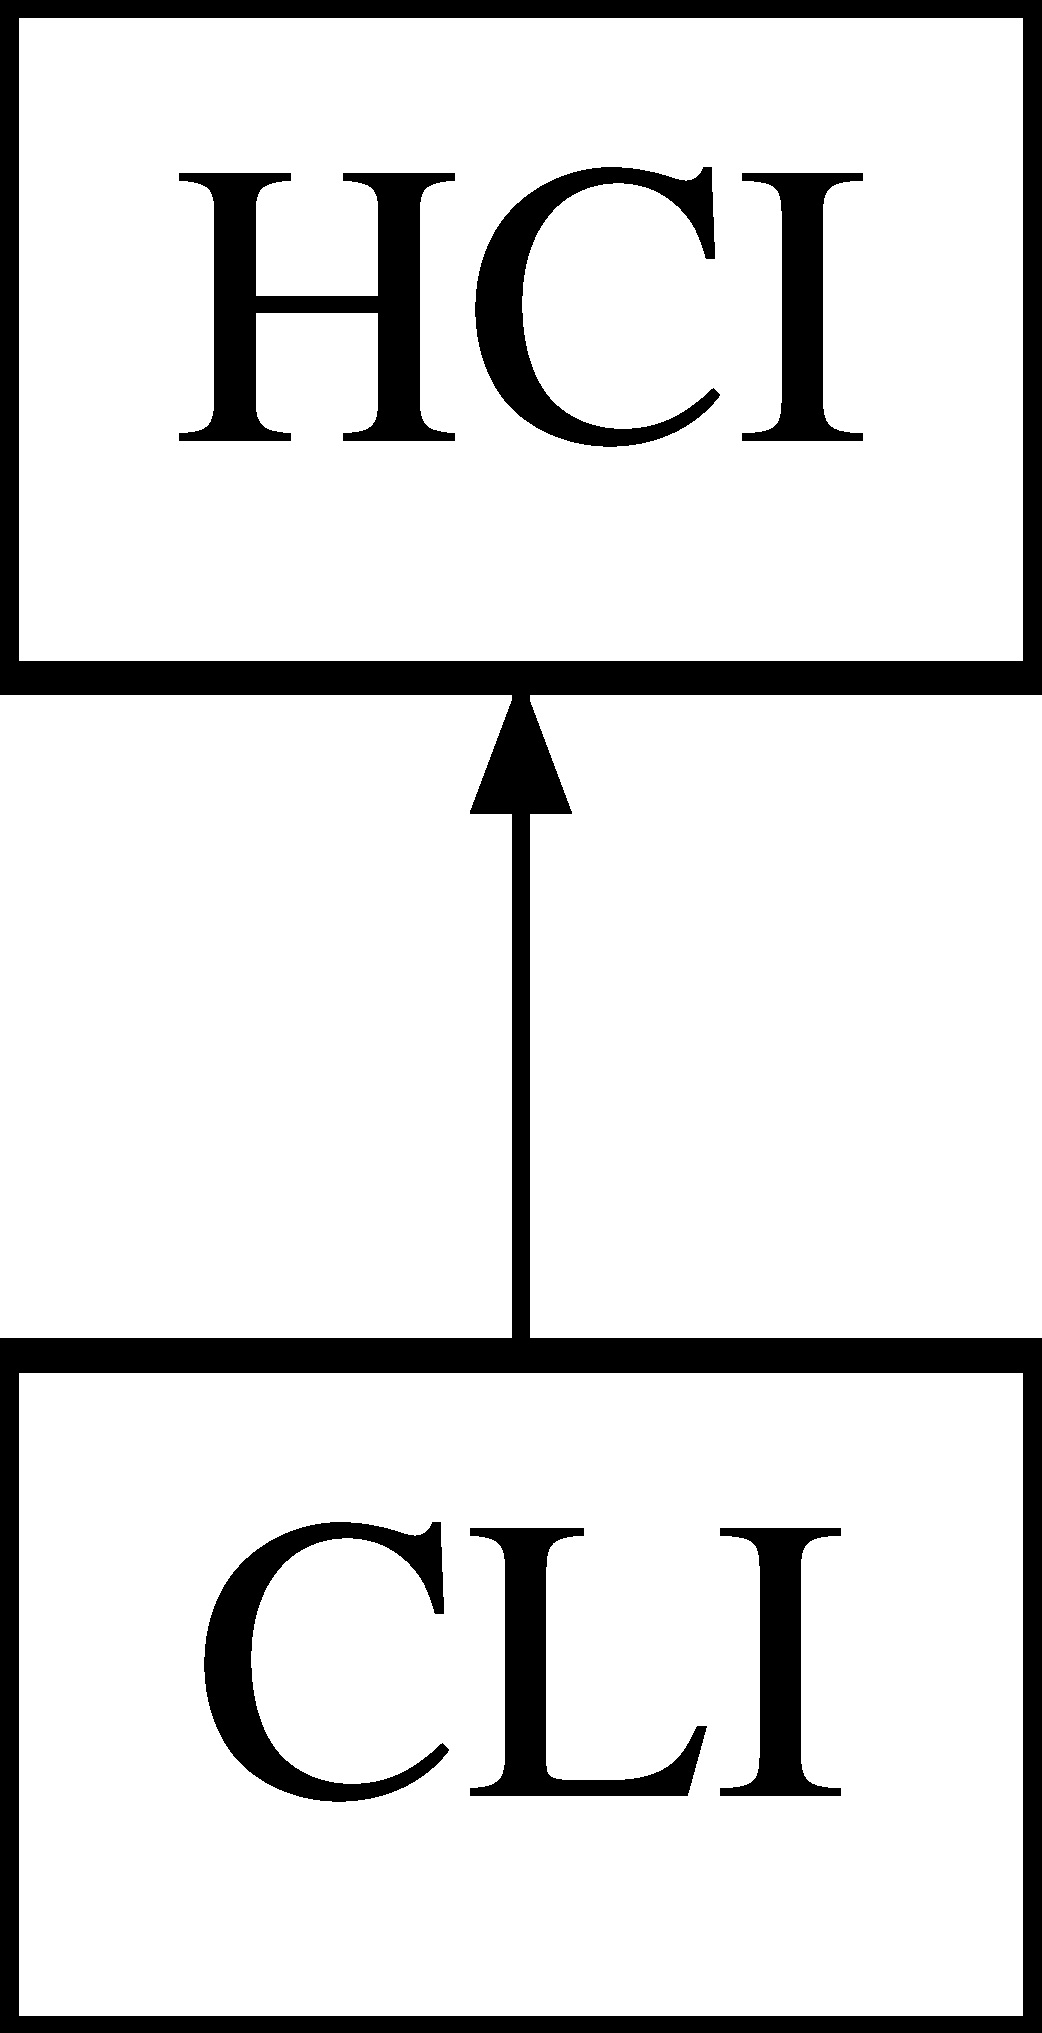
\includegraphics[height=2.000000cm]{classHCI}
\end{center}
\end{figure}
\subsection*{Types publics}
\begin{DoxyCompactItemize}
\item 
enum {\bfseries log\-Level} \{ \\*
{\bfseries N\-O\-T\-H\-I\-N\-G} = -\/1, 
{\bfseries E\-R\-R\-O\-R} = 0, 
{\bfseries W\-A\-R\-N\-I\-N\-G} = 1, 
{\bfseries C\-R\-I\-T\-I\-N\-F\-O} = 2, 
\\*
{\bfseries I\-N\-F\-O} = 3
 \}
\end{DoxyCompactItemize}
\subsection*{Fonctions membres publiques}
\begin{DoxyCompactItemize}
\item 
\hypertarget{classHCI_a3cac51013396bb8a130298a04b966856}{{\bfseries H\-C\-I} (log\-Level=I\-N\-F\-O)}\label{classHCI_a3cac51013396bb8a130298a04b966856}

\item 
\hypertarget{classHCI_ab30b1bd8e7b5ddb8764128e9da1b3062}{void {\bfseries set\-Log\-Level} (log\-Level)}\label{classHCI_ab30b1bd8e7b5ddb8764128e9da1b3062}

\item 
\hypertarget{classHCI_a3ba0116597c8a43a7ceac9639150e6c1}{void {\bfseries log} (log\-Level, std\-::string, bool with\-Time=true) const }\label{classHCI_a3ba0116597c8a43a7ceac9639150e6c1}

\item 
\hypertarget{classHCI_a63e5f2061611136d467cda53e4636713}{virtual void {\bfseries logv} (std\-::string, bool with\-Time) const =0}\label{classHCI_a63e5f2061611136d467cda53e4636713}

\end{DoxyCompactItemize}
\subsection*{Attributs protégés}
\begin{DoxyCompactItemize}
\item 
\hypertarget{classHCI_ac344060f03fa9aa1809cfecb507a83f9}{log\-Level {\bfseries log\-Lev}}\label{classHCI_ac344060f03fa9aa1809cfecb507a83f9}

\end{DoxyCompactItemize}


La documentation de cette classe a été générée à partir des fichiers suivants \-:\begin{DoxyCompactItemize}
\item 
src/\-Core/H\-C\-I.\-h\item 
src/\-Core/H\-C\-I.\-cpp\end{DoxyCompactItemize}

\hypertarget{classIntMessage}{\section{Référence de la classe Int\-Message}
\label{classIntMessage}\index{Int\-Message@{Int\-Message}}
}


Classe de messages contenant entier comme le payload.  




{\ttfamily \#include $<$Int\-Message.\-h$>$}

Graphe d'héritage de Int\-Message\-:\begin{figure}[H]
\begin{center}
\leavevmode
\includegraphics[height=2.000000cm]{classIntMessage}
\end{center}
\end{figure}
\subsection*{Fonctions membres publiques}
\begin{DoxyCompactItemize}
\item 
\hypertarget{classIntMessage_aae52ad3c838b48d6512eea7ffbb89404}{{\bfseries Int\-Message} (std\-::string \hyperlink{classMessage_ac7adddb666acdc47c48f684bd6810a51}{name}, int payload, int time=0)}\label{classIntMessage_aae52ad3c838b48d6512eea7ffbb89404}

\item 
\hypertarget{classIntMessage_a00d3fe88985495e98725c12bfc21c39d}{int \hyperlink{classIntMessage_a00d3fe88985495e98725c12bfc21c39d}{get\-Payload} ()}\label{classIntMessage_a00d3fe88985495e98725c12bfc21c39d}

\begin{DoxyCompactList}\small\item\em Renvoie la charge utile du message. \end{DoxyCompactList}\item 
\hypertarget{classIntMessage_a222a5ba75846757bfc24cea19ce345ed}{std\-::ostream \& \hyperlink{classIntMessage_a222a5ba75846757bfc24cea19ce345ed}{operator$<$$<$} (std\-::ostream \&os)}\label{classIntMessage_a222a5ba75846757bfc24cea19ce345ed}

\begin{DoxyCompactList}\small\item\em Operateur de sortie surchargé \end{DoxyCompactList}\end{DoxyCompactItemize}
\subsection*{Additional Inherited Members}


\subsection{Description détaillée}
Classe de messages contenant entier comme le payload. 

La documentation de cette classe a été générée à partir des fichiers suivants \-:\begin{DoxyCompactItemize}
\item 
src/\-Core/\-Messages/Int\-Message.\-h\item 
src/\-Core/\-Messages/Int\-Message.\-cpp\end{DoxyCompactItemize}

\hypertarget{classISynchronized}{\section{Référence de la classe I\-Synchronized}
\label{classISynchronized}\index{I\-Synchronized@{I\-Synchronized}}
}


Interface pour élément synchronisé  




{\ttfamily \#include $<$I\-Synchronized.\-h$>$}

Graphe d'héritage de I\-Synchronized\-:\begin{figure}[H]
\begin{center}
\leavevmode
\includegraphics[height=3.862069cm]{classISynchronized}
\end{center}
\end{figure}
\subsection*{Fonctions membres publiques}
\begin{DoxyCompactItemize}
\item 
\hypertarget{classISynchronized_af7155c662758d6c70f381bb9b11afcd6}{virtual void \hyperlink{classISynchronized_af7155c662758d6c70f381bb9b11afcd6}{clock} (int time)=0}\label{classISynchronized_af7155c662758d6c70f381bb9b11afcd6}

\begin{DoxyCompactList}\small\item\em Methode appellé à chaque tick d'horloge liée. \end{DoxyCompactList}\end{DoxyCompactItemize}


\subsection{Description détaillée}
Interface pour élément synchronisé 

\begin{DoxyRefDesc}{A faire}
\item[\hyperlink{todo__todo000004}{A faire}]Enventuellement factory de modules ? \end{DoxyRefDesc}


Cette interface vise à homogénéiser la notion de temps (timer) pour les classes qui en dépendent. 

La documentation de cette classe a été générée à partir du fichier suivant \-:\begin{DoxyCompactItemize}
\item 
src/\-Core/I\-Synchronized.\-h\end{DoxyCompactItemize}

\hypertarget{classMacroModule}{\section{Référence de la classe Macro\-Module}
\label{classMacroModule}\index{Macro\-Module@{Macro\-Module}}
}
Graphe d'héritage de Macro\-Module\-:\begin{figure}[H]
\begin{center}
\leavevmode
\includegraphics[height=4.000000cm]{classMacroModule}
\end{center}
\end{figure}
\subsection*{Fonctions membres publiques}
\begin{DoxyCompactItemize}
\item 
\hypertarget{classMacroModule_a138847c1feda40c791d6b88173a23135}{{\bfseries Macro\-Module} (std\-::string=\char`\"{}Default\-Name\char`\"{}, Params=Params())}\label{classMacroModule_a138847c1feda40c791d6b88173a23135}

\item 
\hypertarget{classMacroModule_aa7d592010b740d68028fee87e139ae9f}{\hyperlink{classMacroModule_aa7d592010b740d68028fee87e139ae9f}{Macro\-Module} (std\-::string, \hyperlink{classMemory}{Memory}$<$ int $>$, Params=Params())}\label{classMacroModule_aa7d592010b740d68028fee87e139ae9f}

\begin{DoxyCompactList}\small\item\em Constructeur avec m�moire. \end{DoxyCompactList}\item 
\hypertarget{classMacroModule_a9790fb7c331d99dd03f624b1a5258519}{\hyperlink{classMacroModule_a9790fb7c331d99dd03f624b1a5258519}{$\sim$\-Macro\-Module} ()}\label{classMacroModule_a9790fb7c331d99dd03f624b1a5258519}

\begin{DoxyCompactList}\small\item\em Destructeur. \end{DoxyCompactList}\item 
\hypertarget{classMacroModule_a3c693014fb5e1a46758e7867eca43342}{void {\bfseries add\-Sub\-Module} (\hyperlink{classModule}{Module} $\ast$)}\label{classMacroModule_a3c693014fb5e1a46758e7867eca43342}

\item 
\hypertarget{classMacroModule_ad5aca9e5f7b8784959dae226f845cd20}{void {\bfseries add\-Connexion} (\hyperlink{classConnexion}{Connexion})}\label{classMacroModule_ad5aca9e5f7b8784959dae226f845cd20}

\end{DoxyCompactItemize}
\subsection*{Additional Inherited Members}


La documentation de cette classe a été générée à partir des fichiers suivants \-:\begin{DoxyCompactItemize}
\item 
src/headers/Macro\-Module.\-h\item 
src/includes/Macro\-Module.\-cpp\end{DoxyCompactItemize}

\hypertarget{classMemory}{\section{Référence de la classe Memory}
\label{classMemory}\index{Memory@{Memory}}
}


Repr�sente une m�moire.  




{\ttfamily \#include $<$Memory.\-h$>$}

\subsection*{Fonctions membres publiques}
\begin{DoxyCompactItemize}
\item 
\hypertarget{classMemory_a585d7bb6fc6f2237bcebf94a86b7dd99}{\hyperlink{classMemory_a585d7bb6fc6f2237bcebf94a86b7dd99}{Memory} ()}\label{classMemory_a585d7bb6fc6f2237bcebf94a86b7dd99}

\begin{DoxyCompactList}\small\item\em Constructeur. \end{DoxyCompactList}\item 
\hypertarget{classMemory_a0ffa9759ebbf103f11132a505b93bdc0}{\hyperlink{classMemory_a0ffa9759ebbf103f11132a505b93bdc0}{$\sim$\-Memory} ()}\label{classMemory_a0ffa9759ebbf103f11132a505b93bdc0}

\begin{DoxyCompactList}\small\item\em Destructeur. \end{DoxyCompactList}\end{DoxyCompactItemize}


\subsection{Description détaillée}
Repr�sente une m�moire. 

La m�moire est ici simplement mod�lis�e comme une liste de cl�es et de valeurs, associ�e � des contraintes. 

La documentation de cette classe a été générée à partir des fichiers suivants \-:\begin{DoxyCompactItemize}
\item 
src/headers/Memory.\-h\item 
src/includes/Memory.\-cpp\end{DoxyCompactItemize}

\hypertarget{classMessage}{\section{Référence de la classe Message}
\label{classMessage}\index{Message@{Message}}
}


Classe abstraite de base pour les messages.  




{\ttfamily \#include $<$Message.\-h$>$}

Graphe d'héritage de Message\-:\begin{figure}[H]
\begin{center}
\leavevmode
\includegraphics[height=2.000000cm]{classMessage}
\end{center}
\end{figure}
\subsection*{Fonctions membres publiques}
\begin{DoxyCompactItemize}
\item 
\hypertarget{classMessage_a154809183fa5ec6b5182c487db1167dd}{\hyperlink{classMessage_a154809183fa5ec6b5182c487db1167dd}{Message} (std\-::string \hyperlink{classMessage_ac7adddb666acdc47c48f684bd6810a51}{name}=\char`\"{}Default Name\char`\"{}, int=0)}\label{classMessage_a154809183fa5ec6b5182c487db1167dd}

\begin{DoxyCompactList}\small\item\em Constructeur par défaut. \end{DoxyCompactList}\item 
\hypertarget{classMessage_a3f7275462831f787a861271687bcad67}{virtual \hyperlink{classMessage_a3f7275462831f787a861271687bcad67}{$\sim$\-Message} ()}\label{classMessage_a3f7275462831f787a861271687bcad67}

\begin{DoxyCompactList}\small\item\em Destructeur. \end{DoxyCompactList}\item 
\hypertarget{classMessage_ac03b02000572b0852c574498bf138e87}{std\-::string \hyperlink{classMessage_ac03b02000572b0852c574498bf138e87}{get\-Name} ()}\label{classMessage_ac03b02000572b0852c574498bf138e87}

\begin{DoxyCompactList}\small\item\em Renvoie le nom du message. \end{DoxyCompactList}\item 
\hypertarget{classMessage_acbdab136245666bce3752fa311150672}{virtual std\-::ostream \& \hyperlink{classMessage_acbdab136245666bce3752fa311150672}{operator$<$$<$} (std\-::ostream \&os)=0}\label{classMessage_acbdab136245666bce3752fa311150672}

\begin{DoxyCompactList}\small\item\em Operateur de sortie surchargé \end{DoxyCompactList}\item 
\hypertarget{classMessage_a37550fee6e64d7c83ead2628373f4db3}{unsigned int \hyperlink{classMessage_a37550fee6e64d7c83ead2628373f4db3}{get\-Transmission\-Time} ()}\label{classMessage_a37550fee6e64d7c83ead2628373f4db3}

\begin{DoxyCompactList}\small\item\em Renvoie le temps de traitement du message. \end{DoxyCompactList}\end{DoxyCompactItemize}
\subsection*{Fonctions membres publiques statiques}
\begin{DoxyCompactItemize}
\item 
\hypertarget{classMessage_a18fddc1357914aa65d4a12eeabbf7bfa}{static std\-::shared\-\_\-ptr$<$ \hyperlink{classMessage}{Message} $>$ {\bfseries create\-Message} (std\-::string, int=0, unsigned int=0)}\label{classMessage_a18fddc1357914aa65d4a12eeabbf7bfa}

\item 
\hypertarget{classMessage_a9510bbfbcde96a857eb40b8222fe90a8}{static std\-::shared\-\_\-ptr$<$ \hyperlink{classMessage}{Message} $>$ {\bfseries create\-Message} (std\-::string, std\-::string=\char`\"{}\char`\"{}, unsigned int=0)}\label{classMessage_a9510bbfbcde96a857eb40b8222fe90a8}

\item 
\hypertarget{classMessage_a275c24aa740943af5872d874eeca0173}{static std\-::shared\-\_\-ptr$<$ \hyperlink{classMessage}{Message} $>$ \hyperlink{classMessage_a275c24aa740943af5872d874eeca0173}{create\-Message} (std\-::string, float=0, unsigned=0)}\label{classMessage_a275c24aa740943af5872d874eeca0173}

\begin{DoxyCompactList}\small\item\em Crée et retourne le pointeur partagé au nouveau \hyperlink{classFloatMessage}{Float\-Message}. \end{DoxyCompactList}\end{DoxyCompactItemize}
\subsection*{Attributs protégés}
\begin{DoxyCompactItemize}
\item 
std\-::string \hyperlink{classMessage_ac7adddb666acdc47c48f684bd6810a51}{name}
\item 
unsigned int \hyperlink{classMessage_a9f2d70860e0ec546c8e00cd69a3555ee}{transmission\-Time}
\end{DoxyCompactItemize}


\subsection{Description détaillée}
Classe abstraite de base pour les messages. 

Les messages sont les différentes informations que peuvent se communiquer les modules. Un message est composé de son nom, éventuellement d'une donnée (payload), et d'une indication temporelle concernant la durée de son envoi et de sa réception. 

\subsection{Documentation des données membres}
\hypertarget{classMessage_ac7adddb666acdc47c48f684bd6810a51}{\index{Message@{Message}!name@{name}}
\index{name@{name}!Message@{Message}}
\subsubsection[{name}]{\setlength{\rightskip}{0pt plus 5cm}std\-::string Message\-::name\hspace{0.3cm}{\ttfamily [protected]}}}\label{classMessage_ac7adddb666acdc47c48f684bd6810a51}
Nom du message \hypertarget{classMessage_a9f2d70860e0ec546c8e00cd69a3555ee}{\index{Message@{Message}!transmission\-Time@{transmission\-Time}}
\index{transmission\-Time@{transmission\-Time}!Message@{Message}}
\subsubsection[{transmission\-Time}]{\setlength{\rightskip}{0pt plus 5cm}unsigned int Message\-::transmission\-Time\hspace{0.3cm}{\ttfamily [protected]}}}\label{classMessage_a9f2d70860e0ec546c8e00cd69a3555ee}
Temps de traitement du message 

La documentation de cette classe a été générée à partir des fichiers suivants \-:\begin{DoxyCompactItemize}
\item 
src/\-Core/Message.\-h\item 
src/\-Core/Message.\-cpp\end{DoxyCompactItemize}

\hypertarget{classModule}{\section{Référence de la classe Module}
\label{classModule}\index{Module@{Module}}
}


Les briques de base du simulateur.  




{\ttfamily \#include $<$Module.\-h$>$}

Graphe d'héritage de Module\-:\begin{figure}[H]
\begin{center}
\leavevmode
\includegraphics[height=4.000000cm]{classModule}
\end{center}
\end{figure}
\subsection*{Fonctions membres publiques}
\begin{DoxyCompactItemize}
\item 
\hypertarget{classModule_a3412148164f0668b2ae4cd1285c2790c}{\hyperlink{classModule_a3412148164f0668b2ae4cd1285c2790c}{Module} (std\-::string=\char`\"{}Default\-Name\char`\"{}, Params=Params())}\label{classModule_a3412148164f0668b2ae4cd1285c2790c}

\begin{DoxyCompactList}\small\item\em Constructeur par défault, pour un module sans mémoire. \end{DoxyCompactList}\item 
\hypertarget{classModule_ae2ce24f11deec1453dfaba1f21a36f2c}{\hyperlink{classModule_ae2ce24f11deec1453dfaba1f21a36f2c}{Module} (std\-::string, \hyperlink{classMemory}{Memory}$<$ int $>$, Params=Params())}\label{classModule_ae2ce24f11deec1453dfaba1f21a36f2c}

\begin{DoxyCompactList}\small\item\em Constructeur avec mémoire. \end{DoxyCompactList}\item 
\hypertarget{classModule_a7c9d9c096786d127590fdd8aa2b7d681}{virtual \hyperlink{classModule_a7c9d9c096786d127590fdd8aa2b7d681}{$\sim$\-Module} ()}\label{classModule_a7c9d9c096786d127590fdd8aa2b7d681}

\begin{DoxyCompactList}\small\item\em Destructeur. \end{DoxyCompactList}\item 
virtual void \hyperlink{classModule_ab7ea9648fa500696c85e93ebd0666390}{clock} (int)
\begin{DoxyCompactList}\small\item\em Méthode appellée à chaque pas de temps, commune à tous les modules. \end{DoxyCompactList}\item 
\hypertarget{classModule_aeb7302c667eb923a4dc25ae235c744dc}{void \hyperlink{classModule_aeb7302c667eb923a4dc25ae235c744dc}{add\-Socket} (\hyperlink{classSocket}{Socket})}\label{classModule_aeb7302c667eb923a4dc25ae235c744dc}

\begin{DoxyCompactList}\small\item\em Fonction d'ajout d'un connecteur au module. \end{DoxyCompactList}\item 
\hypertarget{classModule_a7adde67e02dd73bbea1441f7833edc4b}{void \hyperlink{classModule_a7adde67e02dd73bbea1441f7833edc4b}{add\-Message} (\hyperlink{classMessage}{Message}, int)}\label{classModule_a7adde67e02dd73bbea1441f7833edc4b}

\begin{DoxyCompactList}\small\item\em Fonction d'ajout d'un message au module, et de son temps d'éxecution simulé. \end{DoxyCompactList}\item 
\hyperlink{classSocket}{Socket} \& \hyperlink{classModule_a818c5fc693a7ea20db6a2245e94f6561}{get\-Socket\-By\-Name} (std\-::string)
\begin{DoxyCompactList}\small\item\em Récupère le bon connecteur, ou lève une exception. \end{DoxyCompactList}\item 
\hypertarget{classModule_a93e2ee84587751939c1fd31cb0802e41}{double {\bfseries get\-Param\-Value\-By\-Name} (std\-::string)}\label{classModule_a93e2ee84587751939c1fd31cb0802e41}

\item 
\hypertarget{classModule_ace0e4299e1a6f9b46aa9fd316483895d}{void {\bfseries set\-Param\-Value\-By\-Name} (std\-::string, double)}\label{classModule_ace0e4299e1a6f9b46aa9fd316483895d}

\item 
\hypertarget{classModule_ac37dde7b4cbe2ea7b319cd43282296ac}{bool \hyperlink{classModule_ac37dde7b4cbe2ea7b319cd43282296ac}{is\-Message\-Allowed} (\hyperlink{classMessage}{Message})}\label{classModule_ac37dde7b4cbe2ea7b319cd43282296ac}

\begin{DoxyCompactList}\small\item\em Vérifie si le message est un des messages compris par ce module. \end{DoxyCompactList}\end{DoxyCompactItemize}
\subsection*{Attributs protégés}
\begin{DoxyCompactItemize}
\item 
std\-::string \hyperlink{classModule_a794fbb44972c7c73cc197159093e66d1}{name}
\item 
\hyperlink{classMemory}{Memory}$<$ int $>$ \hyperlink{classModule_a48fa02fe55d33daffff725c615a63bb9}{memory}
\item 
Sockets \hyperlink{classModule_af0415ddaab230958f91665c66b078085}{sockets}
\item 
Messages \hyperlink{classModule_aaadd1f971bebf7bb5eae12fcc5689198}{messages\-Allowed}
\item 
Params \hyperlink{classModule_a232443111a9d59c17724992ddf75fbad}{parameters}
\item 
std\-::queue$<$ \hyperlink{classMessage}{Message} $>$ \hyperlink{classModule_aeace7c2bfd88f9946a25fb06974ca522}{tasks}
\item 
int \hyperlink{classModule_afc209c4f9120425219f7775c79cf4bea}{task\-Timer}
\end{DoxyCompactItemize}


\subsection{Description détaillée}
Les briques de base du simulateur. 

Il s'agit de la classe centrale du simulateur, qui sera construit comme un assemblage de modules qui communiquent entre eux. Il s'agit d'une classe virtuelle. 

\subsection{Documentation des fonctions membres}
\hypertarget{classModule_ab7ea9648fa500696c85e93ebd0666390}{\index{Module@{Module}!clock@{clock}}
\index{clock@{clock}!Module@{Module}}
\subsubsection[{clock}]{\setlength{\rightskip}{0pt plus 5cm}void Module\-::clock (
\begin{DoxyParamCaption}
\item[{int}]{time}
\end{DoxyParamCaption}
)\hspace{0.3cm}{\ttfamily [virtual]}}}\label{classModule_ab7ea9648fa500696c85e93ebd0666390}


Méthode appellée à chaque pas de temps, commune à tous les modules. 

Cette méthode effectue trois actions, lire les messages arrivés, avancer dans un processus interne, envoyer un message. Ces actions prennent tous du temps\-: elles peuvent durer plusieurs \char`\"{}ticks\char`\"{}. \begin{DoxyRefDesc}{A faire}
\item[\hyperlink{todo__todo000003}{A faire}]Lever une exception \end{DoxyRefDesc}


Implémente \hyperlink{classISynchronized_af7155c662758d6c70f381bb9b11afcd6}{I\-Synchronized}.

\hypertarget{classModule_a818c5fc693a7ea20db6a2245e94f6561}{\index{Module@{Module}!get\-Socket\-By\-Name@{get\-Socket\-By\-Name}}
\index{get\-Socket\-By\-Name@{get\-Socket\-By\-Name}!Module@{Module}}
\subsubsection[{get\-Socket\-By\-Name}]{\setlength{\rightskip}{0pt plus 5cm}{\bf Socket} \& Module\-::get\-Socket\-By\-Name (
\begin{DoxyParamCaption}
\item[{std\-::string}]{}
\end{DoxyParamCaption}
)}}\label{classModule_a818c5fc693a7ea20db6a2245e94f6561}


Récupère le bon connecteur, ou lève une exception. 

\begin{DoxyRefDesc}{A faire}
\item[\hyperlink{todo__todo000001}{A faire}]Créer et gérer l'exception \end{DoxyRefDesc}
\begin{DoxyRefDesc}{A faire}
\item[\hyperlink{todo__todo000004}{A faire}]Faire le retour d'un objet \end{DoxyRefDesc}


\subsection{Documentation des données membres}
\hypertarget{classModule_a48fa02fe55d33daffff725c615a63bb9}{\index{Module@{Module}!memory@{memory}}
\index{memory@{memory}!Module@{Module}}
\subsubsection[{memory}]{\setlength{\rightskip}{0pt plus 5cm}{\bf Memory}$<$int$>$ Module\-::memory\hspace{0.3cm}{\ttfamily [protected]}}}\label{classModule_a48fa02fe55d33daffff725c615a63bb9}
La mémoire du module \hypertarget{classModule_aaadd1f971bebf7bb5eae12fcc5689198}{\index{Module@{Module}!messages\-Allowed@{messages\-Allowed}}
\index{messages\-Allowed@{messages\-Allowed}!Module@{Module}}
\subsubsection[{messages\-Allowed}]{\setlength{\rightskip}{0pt plus 5cm}Messages Module\-::messages\-Allowed\hspace{0.3cm}{\ttfamily [protected]}}}\label{classModule_aaadd1f971bebf7bb5eae12fcc5689198}
Les messages compris par le module E\-T leurs temps d'éxecution \hypertarget{classModule_a794fbb44972c7c73cc197159093e66d1}{\index{Module@{Module}!name@{name}}
\index{name@{name}!Module@{Module}}
\subsubsection[{name}]{\setlength{\rightskip}{0pt plus 5cm}std\-::string Module\-::name\hspace{0.3cm}{\ttfamily [protected]}}}\label{classModule_a794fbb44972c7c73cc197159093e66d1}
Le nom du module \hypertarget{classModule_a232443111a9d59c17724992ddf75fbad}{\index{Module@{Module}!parameters@{parameters}}
\index{parameters@{parameters}!Module@{Module}}
\subsubsection[{parameters}]{\setlength{\rightskip}{0pt plus 5cm}Params Module\-::parameters\hspace{0.3cm}{\ttfamily [protected]}}}\label{classModule_a232443111a9d59c17724992ddf75fbad}
Les paramètres d'état du modules \hypertarget{classModule_af0415ddaab230958f91665c66b078085}{\index{Module@{Module}!sockets@{sockets}}
\index{sockets@{sockets}!Module@{Module}}
\subsubsection[{sockets}]{\setlength{\rightskip}{0pt plus 5cm}Sockets Module\-::sockets\hspace{0.3cm}{\ttfamily [protected]}}}\label{classModule_af0415ddaab230958f91665c66b078085}
Les connecteurs du module \hypertarget{classModule_aeace7c2bfd88f9946a25fb06974ca522}{\index{Module@{Module}!tasks@{tasks}}
\index{tasks@{tasks}!Module@{Module}}
\subsubsection[{tasks}]{\setlength{\rightskip}{0pt plus 5cm}std\-::queue$<${\bf Message}$>$ Module\-::tasks\hspace{0.3cm}{\ttfamily [protected]}}}\label{classModule_aeace7c2bfd88f9946a25fb06974ca522}
La file d'attente des messages à traiter \hypertarget{classModule_afc209c4f9120425219f7775c79cf4bea}{\index{Module@{Module}!task\-Timer@{task\-Timer}}
\index{task\-Timer@{task\-Timer}!Module@{Module}}
\subsubsection[{task\-Timer}]{\setlength{\rightskip}{0pt plus 5cm}int Module\-::task\-Timer\hspace{0.3cm}{\ttfamily [protected]}}}\label{classModule_afc209c4f9120425219f7775c79cf4bea}
Le timer de la tâche courante 

La documentation de cette classe a été générée à partir des fichiers suivants \-:\begin{DoxyCompactItemize}
\item 
src/headers/Module.\-h\item 
src/includes/Module.\-cpp\end{DoxyCompactItemize}

\hypertarget{classPhysics}{\section{Référence de la classe Physics}
\label{classPhysics}\index{Physics@{Physics}}
}


Classe abstraite pour d�crire les diff�rentes actions de l'environnement sur les modules.  




{\ttfamily \#include $<$Physics.\-h$>$}

Graphe d'héritage de Physics\-:\begin{figure}[H]
\begin{center}
\leavevmode
\includegraphics[height=3.000000cm]{classPhysics}
\end{center}
\end{figure}
\subsection*{Fonctions membres publiques}
\begin{DoxyCompactItemize}
\item 
\hypertarget{classPhysics_a52d941cb606bf293441d2ef0a6a1149c}{{\bfseries Physics} (\hyperlink{classModule}{Module} $\ast$)}\label{classPhysics_a52d941cb606bf293441d2ef0a6a1149c}

\item 
\hypertarget{classPhysics_a041a4739fb28602797808c646c8018fa}{virtual void \hyperlink{classPhysics_a041a4739fb28602797808c646c8018fa}{clock} (int)=0}\label{classPhysics_a041a4739fb28602797808c646c8018fa}

\begin{DoxyCompactList}\small\item\em M�thode appell�e � chaque pas de temps. \end{DoxyCompactList}\end{DoxyCompactItemize}
\subsection*{Attributs protégés}
\begin{DoxyCompactItemize}
\item 
\hypertarget{classPhysics_a925455404c675039ec2dc1ff2d510971}{\hyperlink{classModule}{Module} $\ast$ {\bfseries module}}\label{classPhysics_a925455404c675039ec2dc1ff2d510971}

\end{DoxyCompactItemize}


\subsection{Description détaillée}
Classe abstraite pour d�crire les diff�rentes actions de l'environnement sur les modules. 

Prend en attribut un module dont elle � le droit de changer les param�tres. 

La documentation de cette classe a été générée à partir des fichiers suivants \-:\begin{DoxyCompactItemize}
\item 
src/headers/Physics.\-h\item 
src/includes/Physics.\-cpp\end{DoxyCompactItemize}

\hypertarget{classSocket}{\section{Référence de la classe Socket}
\label{classSocket}\index{Socket@{Socket}}
}


Classe abstraite pour les connecteurs des modules.  




{\ttfamily \#include $<$Socket.\-h$>$}

\subsection*{Types publics}
\begin{DoxyCompactItemize}
\item 
enum {\bfseries stype} \{ {\bfseries I\-N}, 
{\bfseries O\-U\-T}
 \}
\end{DoxyCompactItemize}
\subsection*{Fonctions membres publiques}
\begin{DoxyCompactItemize}
\item 
\hypertarget{classSocket_a7c3256c4fc6e2c603df73201049fae5a}{\hyperlink{classSocket_a7c3256c4fc6e2c603df73201049fae5a}{Socket} ()}\label{classSocket_a7c3256c4fc6e2c603df73201049fae5a}

\begin{DoxyCompactList}\small\item\em Constructeur. \end{DoxyCompactList}\item 
\hypertarget{classSocket_aeac4eb6379a543d38ed88977d3b6630a}{\hyperlink{classSocket_aeac4eb6379a543d38ed88977d3b6630a}{$\sim$\-Socket} ()}\label{classSocket_aeac4eb6379a543d38ed88977d3b6630a}

\begin{DoxyCompactList}\small\item\em Destructeur. \end{DoxyCompactList}\end{DoxyCompactItemize}


\subsection{Description détaillée}
Classe abstraite pour les connecteurs des modules. 

Les sockets mod�lisent les connections entre les modules. Un connecteur peut-\/�tre soit un connecteur d'entr�e, {\itshape In\-Socket}, soit un connecteur de sortie, {\itshape Out\-S\-Ocket}. Les connecteurs sont reli�s entre-\/eux via les objets Connexion. 

La documentation de cette classe a été générée à partir des fichiers suivants \-:\begin{DoxyCompactItemize}
\item 
src/headers/Socket.\-h\item 
src/includes/Socket.\-cpp\end{DoxyCompactItemize}

\hypertarget{classStringMessage}{\section{Référence de la classe String\-Message}
\label{classStringMessage}\index{String\-Message@{String\-Message}}
}


Classe de messages contenant une suite des caractères comme le payload.  




{\ttfamily \#include $<$String\-Message.\-h$>$}

Graphe d'héritage de String\-Message\-:\begin{figure}[H]
\begin{center}
\leavevmode
\includegraphics[height=2.000000cm]{classStringMessage}
\end{center}
\end{figure}
\subsection*{Fonctions membres publiques}
\begin{DoxyCompactItemize}
\item 
\hypertarget{classStringMessage_a205d7c1d64055e34ecd2f3f6664c7e6c}{{\bfseries String\-Message} (std\-::string \hyperlink{classMessage_ac7adddb666acdc47c48f684bd6810a51}{name}, std\-::string payload, int time=0)}\label{classStringMessage_a205d7c1d64055e34ecd2f3f6664c7e6c}

\item 
\hypertarget{classStringMessage_a5c8be5fb2d2d9e78be4e1fc303624610}{std\-::string \hyperlink{classStringMessage_a5c8be5fb2d2d9e78be4e1fc303624610}{get\-Payload} ()}\label{classStringMessage_a5c8be5fb2d2d9e78be4e1fc303624610}

\begin{DoxyCompactList}\small\item\em Renvoie la charge utile du message. \end{DoxyCompactList}\item 
\hypertarget{classStringMessage_a0071398acab934eb263ca6892ea76a4c}{std\-::ostream \& \hyperlink{classStringMessage_a0071398acab934eb263ca6892ea76a4c}{operator$<$$<$} (std\-::ostream \&os)}\label{classStringMessage_a0071398acab934eb263ca6892ea76a4c}

\begin{DoxyCompactList}\small\item\em Operateur de sortie surchargé \end{DoxyCompactList}\end{DoxyCompactItemize}
\subsection*{Additional Inherited Members}


\subsection{Description détaillée}
Classe de messages contenant une suite des caractères comme le payload. 

La documentation de cette classe a été générée à partir des fichiers suivants \-:\begin{DoxyCompactItemize}
\item 
src/\-Core/\-Messages/String\-Message.\-h\item 
src/\-Core/\-Messages/String\-Message.\-cpp\end{DoxyCompactItemize}

\hypertarget{classTimer}{\section{Référence de la classe Timer}
\label{classTimer}\index{Timer@{Timer}}
}


Cette classe sert à la gestion du temps simulé  




{\ttfamily \#include $<$Timer.\-h$>$}

\subsection*{Fonctions membres publiques}
\begin{DoxyCompactItemize}
\item 
\hypertarget{classTimer_aeae0c417d77a86462b51da0615eab8b4}{void \hyperlink{classTimer_aeae0c417d77a86462b51da0615eab8b4}{add} (\hyperlink{classModule}{Module} $\ast$)}\label{classTimer_aeae0c417d77a86462b51da0615eab8b4}

\begin{DoxyCompactList}\small\item\em Ajouter le pointeur au module dans le tableau des modules synchronisés. \end{DoxyCompactList}\item 
\hypertarget{classTimer_a6cc5f746e08a0ec915123ef9687cb691}{void \hyperlink{classTimer_a6cc5f746e08a0ec915123ef9687cb691}{add} (\hyperlink{classPhysics}{Physics} $\ast$)}\label{classTimer_a6cc5f746e08a0ec915123ef9687cb691}

\begin{DoxyCompactList}\small\item\em Ajouter le pointeur au module dans le tableau des modules synchronisés. \end{DoxyCompactList}\item 
\hypertarget{classTimer_a62869fa83e1b76a9ebfe9cca7e56733d}{void \hyperlink{classTimer_a62869fa83e1b76a9ebfe9cca7e56733d}{start} (unsigned int c=100)}\label{classTimer_a62869fa83e1b76a9ebfe9cca7e56733d}

\begin{DoxyCompactList}\small\item\em Lancer le \hyperlink{classTimer}{Timer}. \end{DoxyCompactList}\item 
\hypertarget{classTimer_a63f0eb44b27402196590a03781515dba}{void \hyperlink{classTimer_a63f0eb44b27402196590a03781515dba}{stop} ()}\label{classTimer_a63f0eb44b27402196590a03781515dba}

\begin{DoxyCompactList}\small\item\em Arreter le \hyperlink{classTimer}{Timer}. \end{DoxyCompactList}\item 
\hypertarget{classTimer_a03ffd75bbb89ff1644839523af9fda03}{unsigned int \hyperlink{classTimer_a03ffd75bbb89ff1644839523af9fda03}{get\-Counter} () const }\label{classTimer_a03ffd75bbb89ff1644839523af9fda03}

\begin{DoxyCompactList}\small\item\em Retourne la valeur de compteur. \end{DoxyCompactList}\item 
\hypertarget{classTimer_a7394d4c4edb4d951dbe2c7e1ab2fb7ae}{void \hyperlink{classTimer_a7394d4c4edb4d951dbe2c7e1ab2fb7ae}{set\-Counter} (unsigned int)}\label{classTimer_a7394d4c4edb4d951dbe2c7e1ab2fb7ae}

\begin{DoxyCompactList}\small\item\em Mettre la valeur c dans le compteur. \end{DoxyCompactList}\end{DoxyCompactItemize}
\subsection*{Fonctions membres publiques statiques}
\begin{DoxyCompactItemize}
\item 
\hypertarget{classTimer_a8357f90f20707f9693fc713319de923a}{static \hyperlink{classTimer}{Timer} \& \hyperlink{classTimer_a8357f90f20707f9693fc713319de923a}{get\-Instance} ()}\label{classTimer_a8357f90f20707f9693fc713319de923a}

\begin{DoxyCompactList}\small\item\em Retourne l'instance unique de \hyperlink{classTimer}{Timer}. \end{DoxyCompactList}\end{DoxyCompactItemize}


\subsection{Description détaillée}
Cette classe sert à la gestion du temps simulé 

C'est le timer (unique) qui a pour rôle de synchroniser l'ensemble du simulateur et de donner les informations intéresantes sur le temps simulé. 

La documentation de cette classe a été générée à partir des fichiers suivants \-:\begin{DoxyCompactItemize}
\item 
src/\-Core/Timer.\-h\item 
src/\-Core/Timer.\-cpp\end{DoxyCompactItemize}

\hypertarget{classXMLReader}{\section{Référence de la classe X\-M\-L\-Reader}
\label{classXMLReader}\index{X\-M\-L\-Reader@{X\-M\-L\-Reader}}
}


Classe utilitaire pour la lecture des fichiers de configuration.  




{\ttfamily \#include $<$X\-M\-L\-Reader.\-h$>$}

\subsection*{Fonctions membres publiques}
\begin{DoxyCompactItemize}
\item 
\hypertarget{classXMLReader_a73065c7758f26ef69387e315c96d13ac}{\hyperlink{classXMLReader_a73065c7758f26ef69387e315c96d13ac}{$\sim$\-X\-M\-L\-Reader} ()}\label{classXMLReader_a73065c7758f26ef69387e315c96d13ac}

\begin{DoxyCompactList}\small\item\em Destructeur. \end{DoxyCompactList}\end{DoxyCompactItemize}
\subsection*{Fonctions membres publiques statiques}
\begin{DoxyCompactItemize}
\item 
static std\-::unordered\-\_\-map\\*
$<$ std\-::string, double $>$ \hyperlink{classXMLReader_a176f21253bd7ac73c00c0aa46e2e5724}{read\-Params} (std\-::string)
\begin{DoxyCompactList}\small\item\em Lecture des paramètre du module protant ce nom. Cette fonction recherche le fichier de configuration portant le nom du module, appelle le parser Rapid\-X\-M\-L puis créé le tableau de paramètres. En cas d'échec, elle lève une exception. \end{DoxyCompactList}\item 
\hypertarget{classXMLReader_aa21f5dcd9d009e635c6acad97beb240a}{static std\-::unordered\-\_\-map\\*
$<$ std\-::string, int $>$ \hyperlink{classXMLReader_aa21f5dcd9d009e635c6acad97beb240a}{read\-Messages} (std\-::string)}\label{classXMLReader_aa21f5dcd9d009e635c6acad97beb240a}

\begin{DoxyCompactList}\small\item\em Lecture des méssages compris par le module protant ce nom. Cette fonction recherche le fichier de configuration portant le nom du module, appelle le parser Rapid\-X\-M\-L puis créé le tableau de messages. En cas d'échec, elle lève une exception. \end{DoxyCompactList}\item 
\hypertarget{classXMLReader_af23225be3e3a4db017f1e22d1b21f7eb}{static std\-::vector$<$ std\-::string $>$ \hyperlink{classXMLReader_af23225be3e3a4db017f1e22d1b21f7eb}{read\-Sockets} (std\-::string)}\label{classXMLReader_af23225be3e3a4db017f1e22d1b21f7eb}

\begin{DoxyCompactList}\small\item\em Lecture des sockets de modile portant ce nom. Cette fonction recherche le fichier de configuration portant le nom du module, appelle le parser Rapid\-X\-M\-L puis créé le tableau de noms de sockets. En cas d'échec, elle lève une exception. \end{DoxyCompactList}\item 
\hypertarget{classXMLReader_a5147abbb0cacd3fbcc396a23cc63456b}{static std\-::string \hyperlink{classXMLReader_a5147abbb0cacd3fbcc396a23cc63456b}{get\-Path} ()}\label{classXMLReader_a5147abbb0cacd3fbcc396a23cc63456b}

\begin{DoxyCompactList}\small\item\em Getter statique du chemin vers le dossier de configuration. \end{DoxyCompactList}\item 
\hypertarget{classXMLReader_ae8d2d4fd99c45bc46b939d9dc3548340}{static void \hyperlink{classXMLReader_ae8d2d4fd99c45bc46b939d9dc3548340}{set\-Path} (std\-::string)}\label{classXMLReader_ae8d2d4fd99c45bc46b939d9dc3548340}

\begin{DoxyCompactList}\small\item\em Setter statique du chemin vers le dossier de configuration. \end{DoxyCompactList}\end{DoxyCompactItemize}


\subsection{Description détaillée}
Classe utilitaire pour la lecture des fichiers de configuration. 

Cette classe statique fournit des méthodes statiques permettant par exemple de lire la configuration initiale du simulateur dans les fihciers xml 

\subsection{Documentation des fonctions membres}
\hypertarget{classXMLReader_a176f21253bd7ac73c00c0aa46e2e5724}{\index{X\-M\-L\-Reader@{X\-M\-L\-Reader}!read\-Params@{read\-Params}}
\index{read\-Params@{read\-Params}!XMLReader@{X\-M\-L\-Reader}}
\subsubsection[{read\-Params}]{\setlength{\rightskip}{0pt plus 5cm}static std\-::unordered\-\_\-map$<$ std\-::string, double $>$ X\-M\-L\-Reader\-::read\-Params (
\begin{DoxyParamCaption}
\item[{std\-::string}]{module\-Name}
\end{DoxyParamCaption}
)\hspace{0.3cm}{\ttfamily [static]}}}\label{classXMLReader_a176f21253bd7ac73c00c0aa46e2e5724}


Lecture des paramètre du module protant ce nom. Cette fonction recherche le fichier de configuration portant le nom du module, appelle le parser Rapid\-X\-M\-L puis créé le tableau de paramètres. En cas d'échec, elle lève une exception. 

Le chemin vers le dossier de configuration 

La documentation de cette classe a été générée à partir des fichiers suivants \-:\begin{DoxyCompactItemize}
\item 
src/\-Core/X\-M\-L\-Reader.\-h\item 
src/\-Core/X\-M\-L\-Reader.\-cpp\end{DoxyCompactItemize}

%--- End generated contents ---

% Index
\newpage
\phantomsection
\addcontentsline{toc}{chapter}{Index}
\printindex

\end{document}
